\section{Implementation}\label{sec:impl}

This section introduces our implementation $\tool$, an extension of a
state-of-the-art JavaScript conformance test synthesizer $\jest$~\cite{jest},
that supports both $k$-FS and $k$-FCPS coverage criteria.
%
Then, we explain how to detect conformance in JavaScript engines and transpilers
using the synthesized conformance tests.

%----------------------------------------%
%----------------------------------------%

\subsection{Overall Structure}\label{sec:overall}

\begin{figure}
  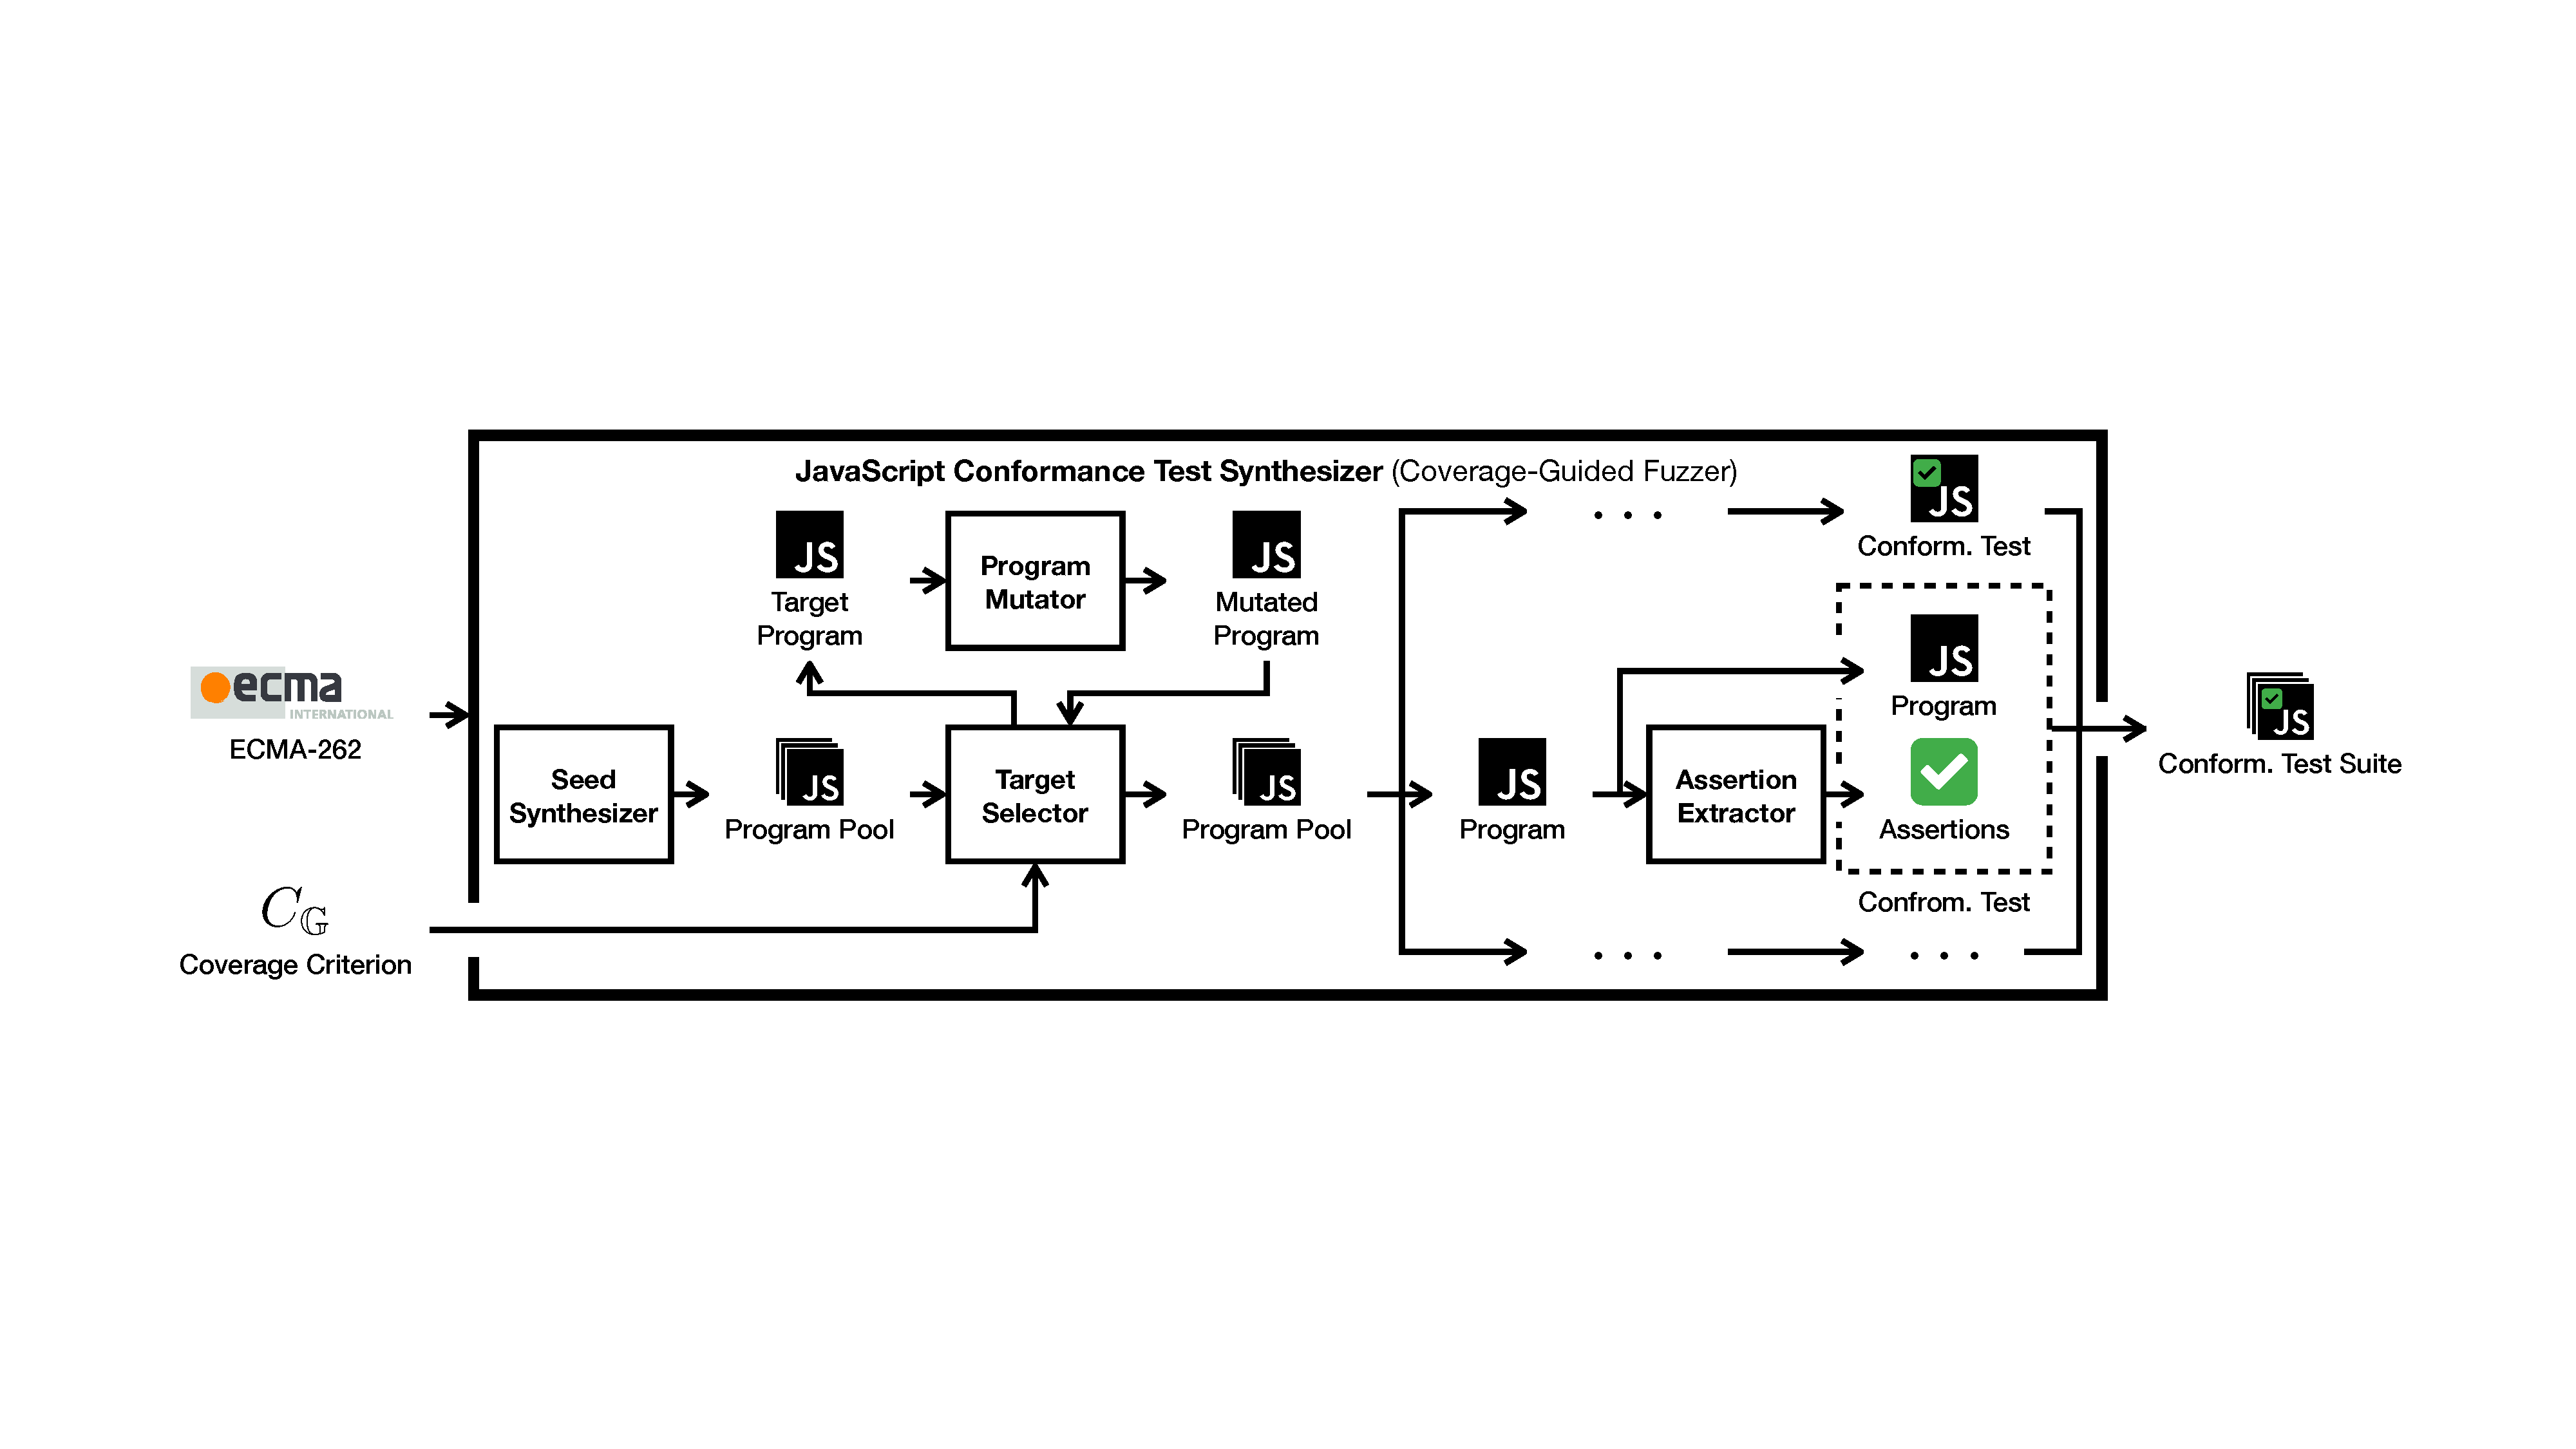
\includegraphics[width=\textwidth]{img/overall}
  \caption{
    Overall structure of a JavaScript conformance test synthesizer using
    coverage-guided fuzzing using the CFG of a mechanized specification
    extracted from the language specification, ECMA-262.
  }
  \label{fig:overall}
\end{figure}

%----------------------------------------%

First, we describe the overall structure of $\tool$ and explain which parts are
updated compared to the baseline tool.
%
$\jest$ is a state-of-the-art JavaScript conformance synthesizer using
coverage-guided fuzzing~\cite{afl} using the CFG in the language specification.
%
It utilizes another tool $\jiset$~\cite{jiset} to automatically extract a
mechanized specification directly from a given version of ECMA-262.
%
We extend $\jest$ to support both $k$-FS and $k$-FCPS coverage criteria.
%
Note that $\jest$ is recently updated based on $\esmeta$, a re-branded version
of $\jiset$ becuase it is deprecated now.\footnote{
  See \url{https://github.com/es-meta/esmeta}
}
%
As depicted in Figure~\ref{fig:overall}, it takes 1) the mechanized
specification for JavaScript, and 2) a coverage criterion $\cov{\graph}$ for CFG
of the specification.
%
We mark the extended part compared to the baseline as red to highlight.

$\tool$ consists of four modules that mechanically utilize JavaScript syntax and
semantics described in the given language specification.
\begin{itemize}
  \item \textsf{\textbf{Seed Synthesizer}}:
    %
    As the first step, \textsf{Seed Synthesizer} automatically synthesizes a set
    of JavaScript programs as the initial \textit{program pool}.
    %
    It utilizes JavaScript syntax described in the language specification to
    cover diverse alternatives in syntactic productions as much as possible.
    %
    Our tool uses existing two synthesizers: 1) a non-recursive synthesizer and
    2) a built-in synthesizer.
    %
  \item \textsf{\textbf{Target Selector}}:
    %
    To measure the coverage in the CFG, \textsf{Target Selector} extracts the
    execution path of each program in the pool by interpreting it using the
    abstract algorithms in the specification.
    %
    While the baseline tool supports only a node-or-branch coverage criterion,
    we extend it to support $k$-FS and $k$-FCPS node-or-branch coverage
    criteria as well.
    %
    If a program does not cover new TRs, it removes the program from the pool.
    %
    Then, it selects a program as a mutation target in the pool that potentially
    increases the coverage or stops the iteration when the current status
    satisfies the termination condition.
    %
  \item \textsf{\textbf{Program Mutator}}:
    %
    To increase the coverage in the CFG, \textsf{Program Mutator} repeatedly
    tries to mutate a JavaScript program to a new one based on mutation methods.
    %
    Our tool uses five existing mutation methods: 1) a random mutation, 2)
    nearest syntax tree mutation, 3) string substitution, 4) object
    substitution, and 5) statement insertion.
    %
  \item \textsf{\textbf{Assertion Extractor}}:
    %
    After the mutation iteration, \textsf{Assertion Extractor} automatically
    extracts seven kinds of assertions from each program in the pool.
    %
    The assertions represent the expected final state of each program according
    to the semantics described in the specification.
    %
    As a result, each pair of a program and the corresponding extracted
    assertions is a \textit{conformance test} for JavaScript.
\end{itemize}

%----------------------------------------%

\begin{figure}
  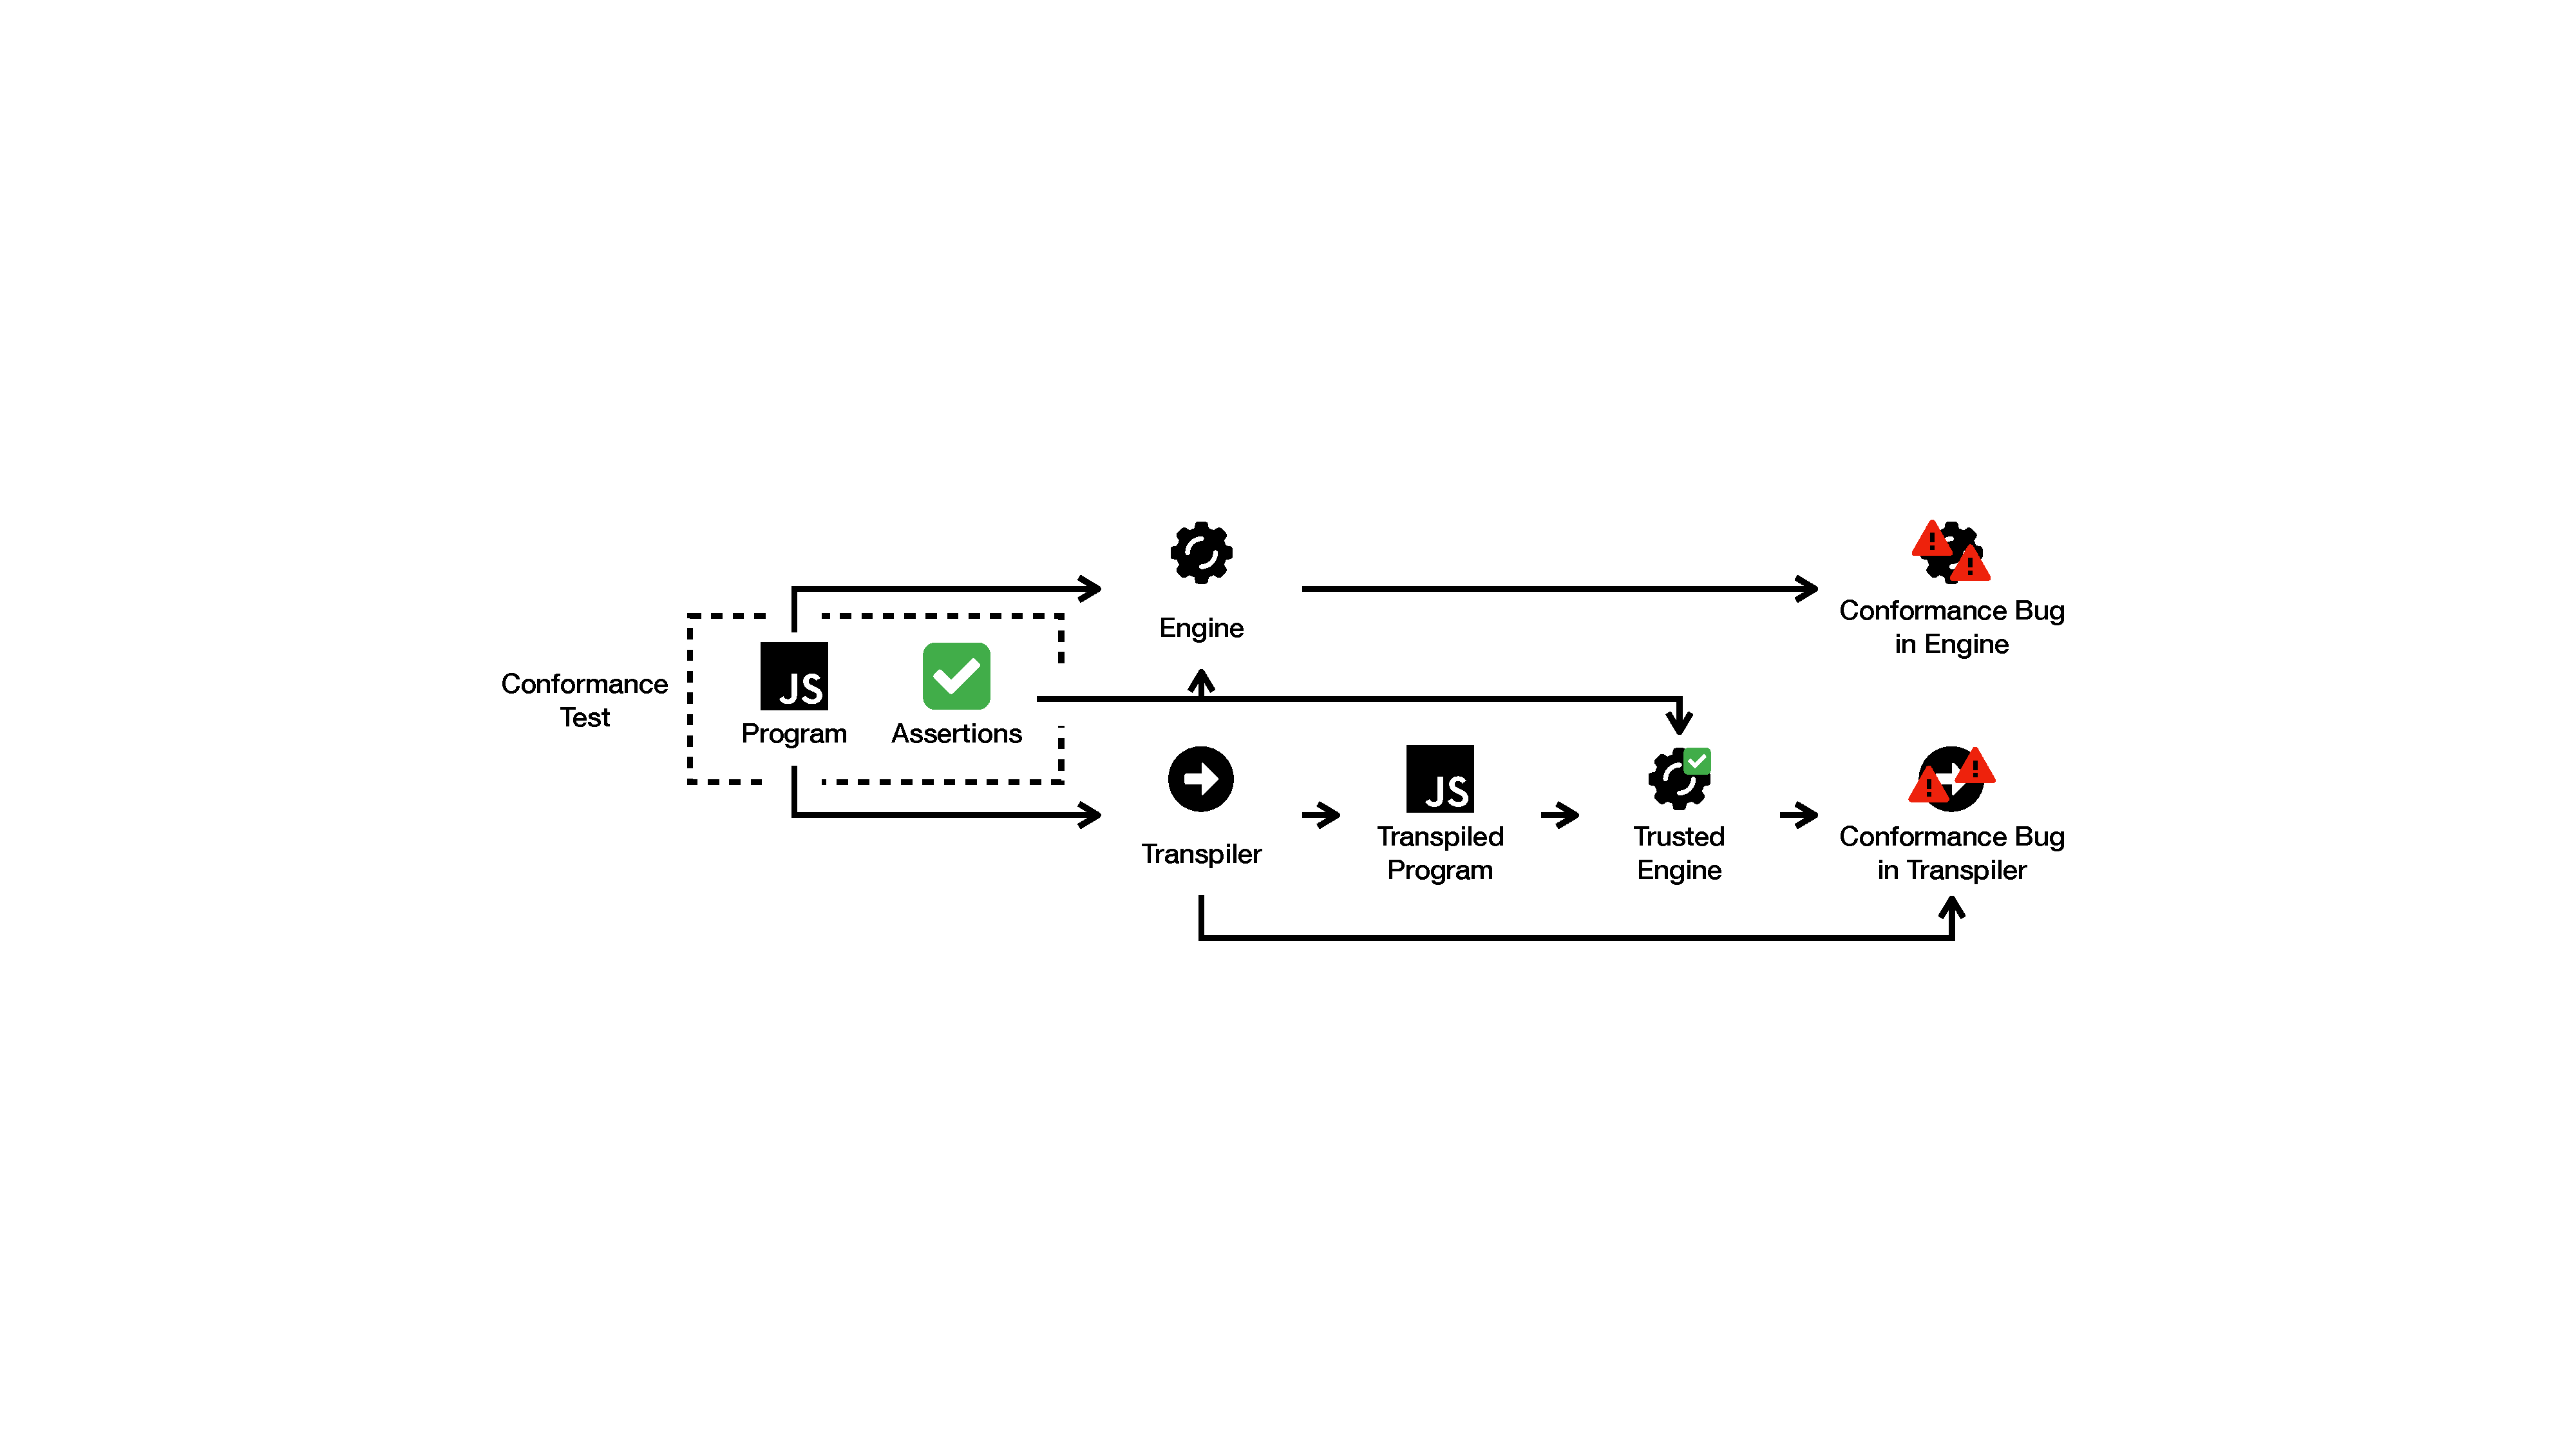
\includegraphics[width=\textwidth]{img/conform-check}
  \caption{
    Conformance check of both engines and transpilers with synthesized
    conformance tests.
  }
  \label{fig:conform-check}
\end{figure}

%----------------------------------------%
%----------------------------------------%

\paragraph{\textbf{Conformance Check of Engines and Transpilers}}
%
A synthesized conformance test consists of a JavaScript program and
corresponding assertions.
%
Figure~\ref{fig:conform-check} depicts how to use it to check the conformance of
JavaScript engines and transpilers.
%
First, assume that we want to check the conformance of a JavaScript engine.
%
In this case, it is enough to run the program and assertions together in the
target engine.
%
Then, if at least one assertion fails, we know the target engine has a
conformance bug related to the test.

On the other hand, we should transpile the program in the test for JavaScript
transpilers.
%
If the target transpiler abnormally terminates, it is a conformance bug because
the program of each conformance test is valid.
%
Otherwise, we should run the transpiled program and assertions together using an
engine.
%
Note that a trusted or already tested JavaScript engine is required to check the
conformance of the transpiler correctly.
%
Like the engine conformance check, the target transpiler has a conformance bug
related to the test if at least one assertion fails.
